\documentclass[a4paper, 11pt]{article}
\usepackage{covington}
\usepackage{amssymb}
\usepackage{amsmath}
\usepackage{hyperref}
%\usepackage{cmbright}
%\usepackage[math]{anttor}
%\usepackage{pxfonts}
\usepackage{mathpazo}
%\usepackage{mathpple}
\usepackage[catalan]{babel}
\usepackage{graphicx}
\usepackage{eurosym}
\usepackage{dsfont}
\usepackage{color}
\usepackage[utf8]{inputenc}
\usepackage{fancyvrb}
\usepackage[usenames,dvipsnames]{xcolor}
\textheight=23.94cm 
\textwidth=17cm 
\topmargin=-1cm 
\oddsidemargin=-0.5cm 

\newcommand{\header}[2]{
\begin{flushleft}
		\rule{\linewidth}{0.6pt}
		\vspace{0.01cm}
		
		{\large{#1}}\\
		\vspace{0.1in}
		{#2}\\
		\vspace{0.1in}
		
		\rule{\linewidth}{0.6pt}
\end{flushleft}
}

\newcommand{\norm}[1]{\left\lVert#1\right\rVert}

\begin{document}
\header{\textbf{Text Mining $-$ Assignment \#2}}{Roger Cuscó, Matthew-Sudmann-Day and Miquel Torrens}
%%%%%%%%%%%%%%%%%%%%
\textbf{\underline{Exercise 1}}\\
\newline We constructed a TF-IDF matrix for the full corpus of the State of the Union speeches dataset. We extracted subsets of those documents based on characteristics that we believe could affect the content. Then we performed a cosine similarity comparison between documents within each subset and between the two subsets. This will tell us whether or not the characteristics we have chosen for categorizing the documents are reflected in term frequencies.\\
\newline We can perform the above analysis directly as described or we can reduce noise in the data by performing a singular value decomposition (SVD), replacing the smaller singular values with zeros, and then recomposing. Selecting a ``reasonable" number of singular values to retain is not necessarily easy so we plotted results against a variety of singular values, in increments of 10.\\
\newline On the plots below, the $x$-axis shows the number of singular values retained. Zero was preserved as a special value meaning that no SVD was performed so the analysis was explicitly done against the original TF-IDF matrix in that one case. One can easily observe, unsurprisingly, that when we retrain \textbf{all} singular values, the result is the same as if the SVD was not performed at all. This explains why the left edge and the right edge of the plots look identical.\\
\newline First, observe a breakdown by party. As you can see, the number of retained singular values changes the conclusions but only at the extreme. As long as we eliminate a few singular values, we eliminate enough noise. And we conclude that SoU speeches of Republicans are more similar to each other than those of Democrats. But they are both more similar to each other than they are to speeches from presidents of the other party.
\begin{center}
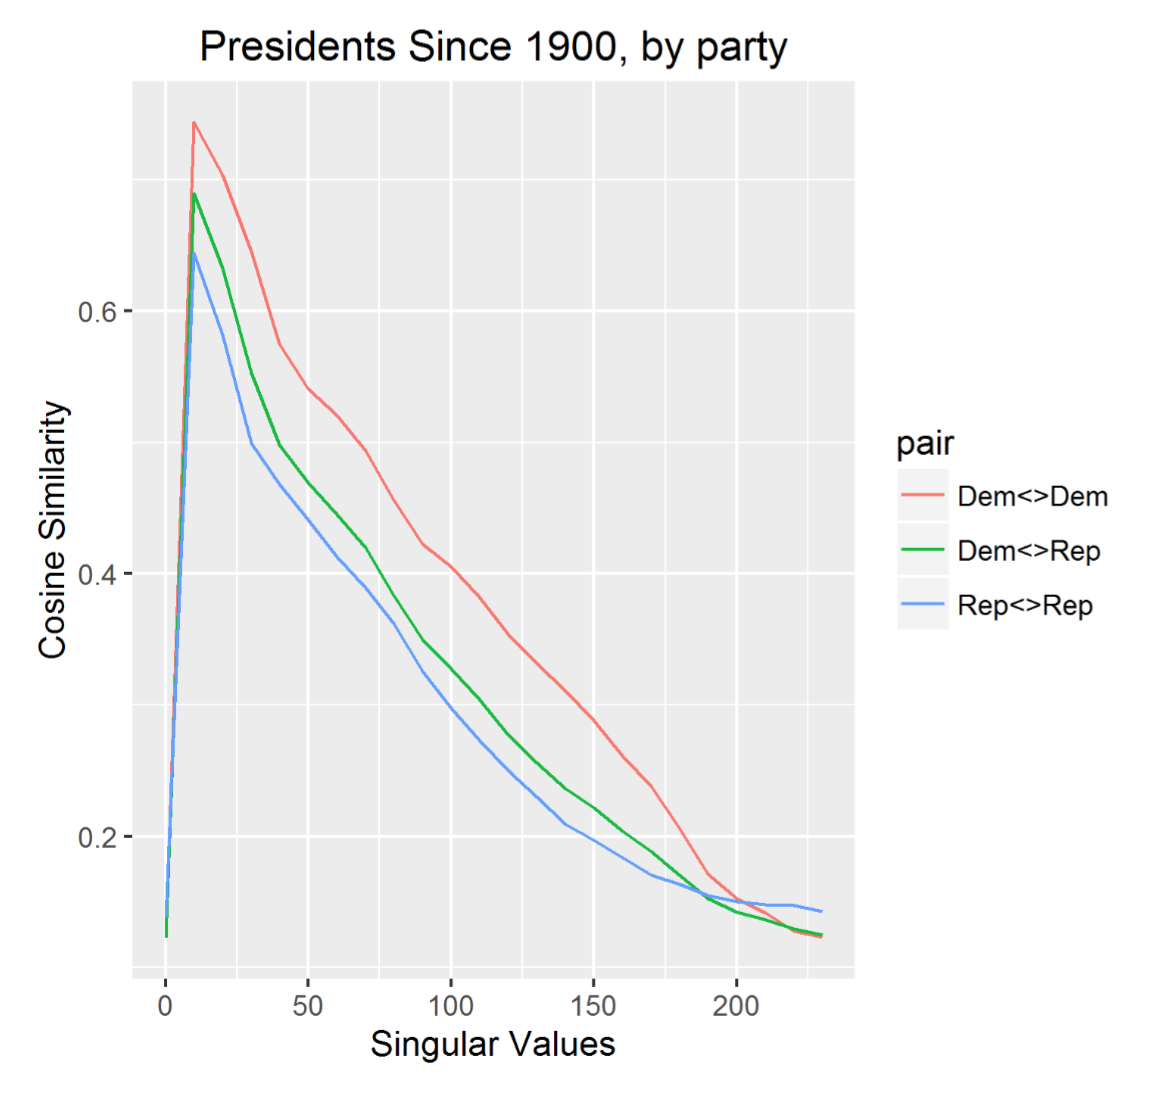
\includegraphics[scale=0.45]{plot1.png}
\end{center}
For those who have been alive in the last 16 years, the follow is a very intuitive result is below: speeches of Bush (W) have a character that is easily identified as different from those of Obama. However, retaining too many or too few singular values will tell us that Obama’s speeches more resemble each other than Bush’s do. Retaining a medium or “reasonable” number will tell us the opposite.
\begin{center}
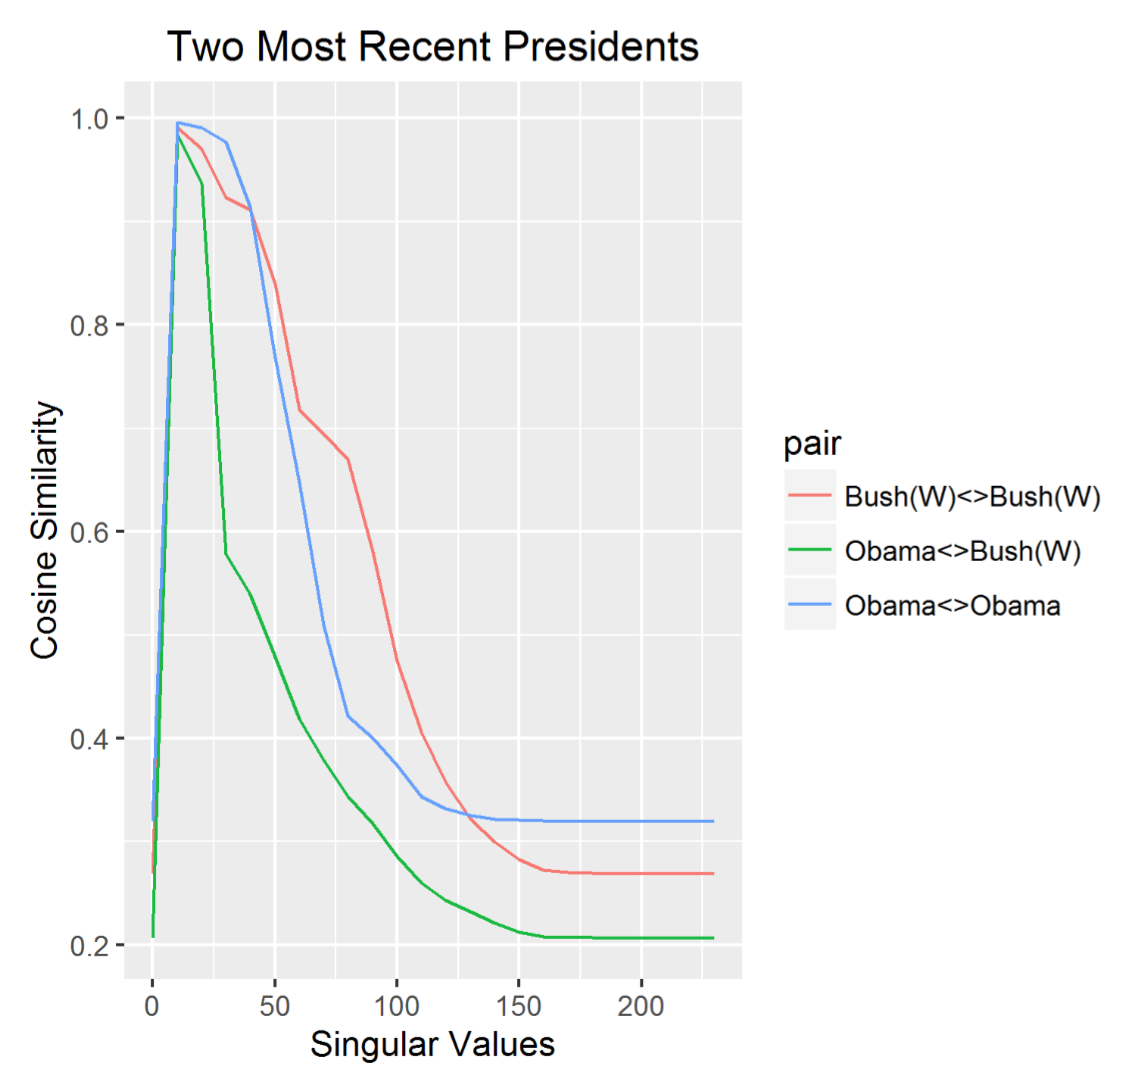
\includegraphics[scale=0.45]{plot2.png}
\end{center}
Finally, the language and politics evolves enough over the centuries to easily separate 19\textsuperscript{th} century and 20\textsuperscript{th} century speeches, regardless of the party of the president.
\begin{center}
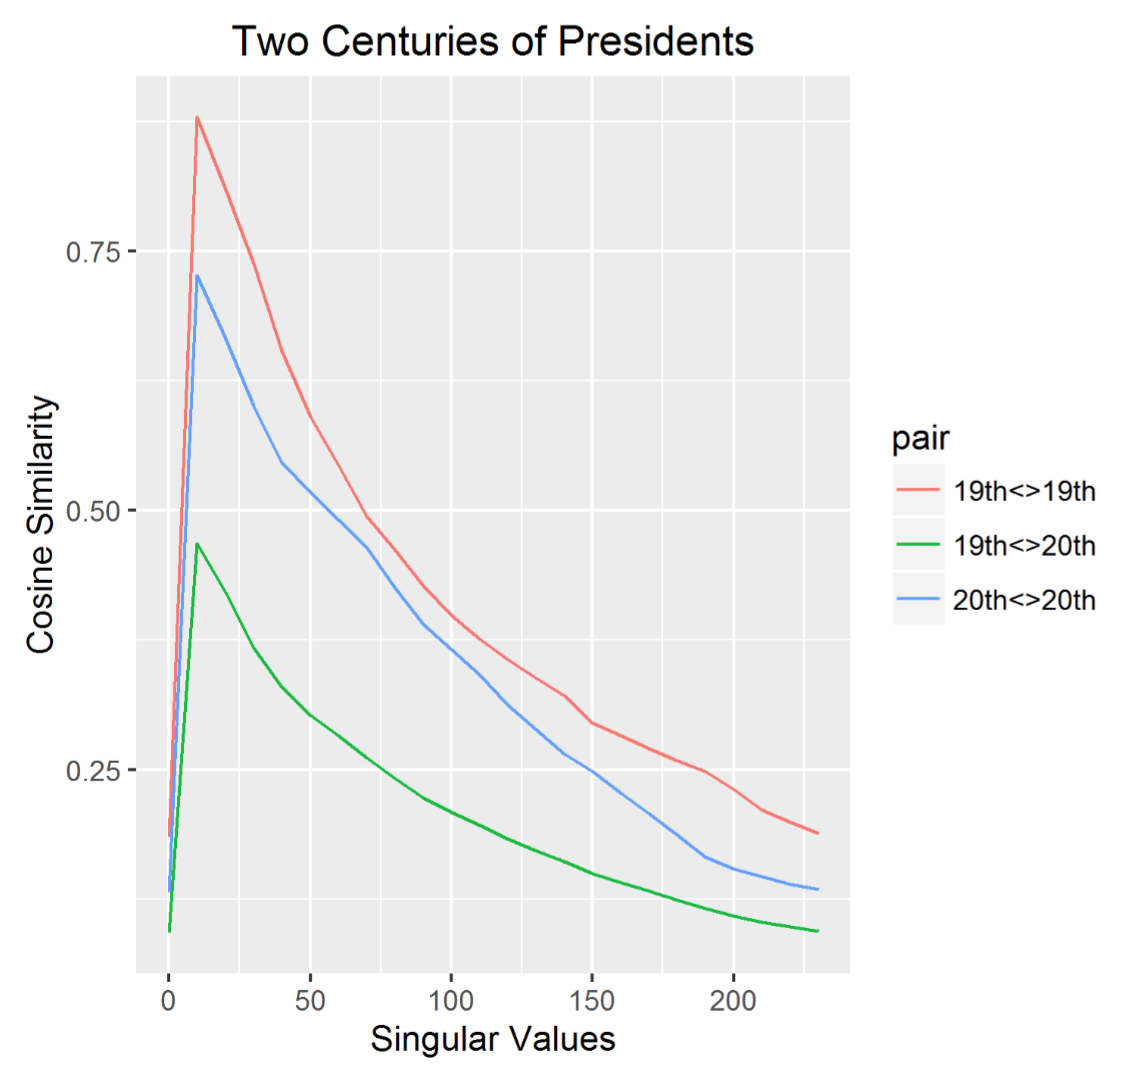
\includegraphics[scale=0.45]{plot3.png}
\end{center}
%%%%%%%%%%%%%%%%%%%%
\pagebreak
\textbf{\underline{Exercise 2}}\\
\newline \textbf{Part (a)}\\
%\newline The parameters of the model are $K$, $\rho_k$ for $k \in \{ 1, \dots, K \}$, $\beta_{z_i}^{1} \in \Delta^{V_1 - 1}$ and $\beta_{z_i}^{2} \in \Delta^{V_2 - 1}$. The latent variables are all $z_i$, for all $i$'s. The observed data are $x_i^{(1)} = (x_{i1}^{(1)}, \dots, x_{iv}^{(1)}, \dots, x_{iV_1}^{(1)}) \in \mathbb{R}^{V_1}$  and $x_i^{(2)} = (x_{i1}^{(2)}, \dots, x_{iv}^{(2)}, \dots, x_{iV_2}^{(2)}) \in \mathbb{R}^{V_2}$.
\newline The components of the model are the following:
\begin{itemize}
\item Parameters:
\begin{itemize}
\item $\pmb{\rho} = ( \rho_1, \dots, \rho_k, \dots, \rho_K ) \in \mathbb{R}^K$
\item $\mathbf{B}^{(1)} = \left( \beta_{z_1}^{(1)}, \dots, \beta_{z_i}^{(1)}, \dots, \beta_{z_N}^{(1)} \right)$, where $\beta_{z_i}^{(1)} \in \Delta^{V_1 - 1}$, $\forall i$
\item $\mathbf{B}^{(2)} = \left( \beta_{z_1}^{(2)}, \dots, \beta_{z_i}^{(2)}, \dots, \beta_{z_N}^{(2)} \right)$, where $\beta_{z_i}^{(2)} \in \Delta^{V_2 - 1}$, $\forall i$
\end{itemize}
For notational purposes, let $\mathbf{B} = \{ \mathbf{B}^{(1)}, \mathbf{B}^{(2)} \}$.
\item Latent variables:
\begin{itemize}
\item $\mathbf{z} = (z_1, \dots, z_i, \dots, z_N) \in \mathbb{R}^{N}$, for $i \in \{ 1, \dots, N \}$ observations
\end{itemize}
\item Observed data:
\begin{itemize}
\item $\mathbf{x}_i^{(1)} = \left( x_{i1}^{(1)}, \dots, x_{iv_1}^{(1)}, \dots, x_{iV_1}^{(1)} \right) \in \mathbb{R}^{V_1}$, $\forall i \in \{ 1, \dots, N \}$
\item $\mathbf{x}_i^{(2)} = \left( x_{i1}^{(2)}, \dots, x_{iv_2}^{(2)}, \dots, x_{iV_2}^{(2)} \right) \in \mathbb{R}^{V_2}$, $\forall i \in \{ 1, \dots, N \}$
\end{itemize}
For notational purposes, let $\mathbf{x}_i = \left\{ \mathbf{x}_i^{(1)}, \mathbf{x}_i^{(2)} \right\} \forall i$ and $\mathbf{x} = \{ \mathbf{x}_1, \dots, \mathbf{x}_i, \dots, \mathbf{x}_N \}$.
\end{itemize}
\textbf{Part (b)}\\
\newline The density function is:
\begin{eqnarray}
\mathbb{P}\left( \mathbf{x}_i | \pmb{\rho}, \mathbf{B} \right) &=& \mathbb{P}\left( \mathbf{x}_i^{(1)}, \mathbf{x}_i^{(2)} | \pmb{\rho}, \mathbf{B} \right) \nonumber \\
&=& \mathbb{P}\left(\mathbf{x}_i^{(1)} | \pmb{\rho}, \mathbf{B}\right)\mathbb{P}\left(\mathbf{x}_i^{(2)} | \pmb{\rho}, \mathbf{B}\right)\hspace{0.5cm} \text{(By independence of the two vectors)} \nonumber \\
&=& \sum_{k=1}^{K} \mathbb{P}\left(z_k | \pmb{\rho}, \mathbf{B}\right)\mathbb{P}\left(\mathbf{x}_i^{(1)} | z_k, \pmb{\rho}, \mathbf{B}\right)\mathbb{P}\left(\mathbf{x}_i^{(2)} | z_k, \pmb{\rho}, \mathbf{B}\right)\nonumber \\
&=& \sum_{k=1}^{K} \rho_k \mathbb{P}\left(\mathbf{x}_i^{(1)} | z_k, \pmb{\rho}, \mathbf{B}\right)\mathbb{P}\left(\mathbf{x}_i^{(2)} | z_k, \pmb{\rho}, \mathbf{B}\right)\nonumber \\
&=& \sum_{k=1}^{K} \rho_k \prod_{v_1=1}^{V_1} \left( \beta_{z_i v_1}^{(1)} \right)^{x_{i v_1}^{(1)}} \prod_{v_2=1}^{V_2} \left( \beta_{z_i v_2}^{(2)} \right)^{x_{i v_2}^{(2)}}. \nonumber
\end{eqnarray}
The likelihood function is the joint probability of all $\mathbf{x}_i$'s:
\begin{eqnarray}
\ell (\mathbf{x} | \pmb{\rho}, \mathbf{B}) = \prod_{i=1}^N \sum_{k=1}^{K} \rho_k \prod_{v_1=1}^{V_1} \left( \beta_{z_i v_1}^{(1)} \right)^{x_{i v_1}^{(1)}} \prod_{v_2=1}^{V_2} \left( \beta_{z_i v_2}^{(2)} \right)^{x_{i v_2}^{(2)}}. \nonumber
\end{eqnarray}
The complete likelihood incorporates the latent variable and writes as follows:
\begin{eqnarray}
\ell_{\text{comp}} (\mathbf{x}, \mathbf{z} | \pmb{\rho}, \mathbf{B}) = \prod_{i=1}^N \prod_{k=1}^{K} \left[ \rho_k \prod_{v_1=1}^{V_1} \left( \beta_{z_i v_1}^{(1)} \right)^{x_{i v_1}^{(1)}} \prod_{v_2=1}^{V_2} \left( \beta_{z_i v_2}^{(2)} \right)^{x_{i v_2}^{(2)}} \right]^{\mathbb{1}_{ \left\{ z_i = k \right\} }}. \nonumber
\end{eqnarray}
Finally, the complete log-likelihood gives:
\begin{eqnarray}
\log \ell_{\text{comp}} (\mathbf{x}, \mathbf{z} | \pmb{\rho}, \mathbf{B}) = \sum_{i=1}^N \sum_{k=1}^{K} \mathbb{1}_{ \left\{ z_i = k \right\} } \left[ \log \rho_k + \sum_{v_1=1}^{V_1} x_{i v_1}^{(1)} \log \beta_{z_i v_1}^{(1)} + \sum_{v_2=1}^{V_2} x_{i v_2}^{(2)} \log \beta_{z_i v_2}^{(2)} \right]. \nonumber
\end{eqnarray}
\newline \textbf{Part (c)}\\
\newline Denote the function $Q$ as:
\begin{eqnarray}
Q(\pmb{\rho}, \mathbf{B}) = \sum_{i=1}^N \sum_{k=1}^{K} \hat{z}_{i,k} \left[ \log \rho_k + \sum_{v_1=1}^{V_1} x_{i v_1}^{(1)} \log \beta_{z_i v_1}^{(1)} + \sum_{v_2=1}^{V_2} x_{i v_2}^{(2)} \log \beta_{z_i v_2}^{(2)} \right], \label{Qfunc}
\end{eqnarray}
where using the Bayes' rule:
\begin{eqnarray}
\hat{z}_{i,k} \equiv \mathbb{E}\left[\mathbb{1}_{ \left\{ z_i = k \right\} } | \pmb{\rho}, \mathbf{B}, \mathbf{x}_i \right] &=& \mathbb{P}\left( z_i = k  | \pmb{\rho}, \mathbf{B}, \mathbf{x}_i \right) \nonumber \\
&\propto& \mathbb{P}\left( \mathbf{x}_i | \pmb{\rho}, \mathbf{B}, z_i = k \right) \mathbb{P}\left( z_i = k | \pmb{\rho}, \mathbf{B} \right) \nonumber \\
&=& \rho_k \prod_{v_1=1}^{V_1} \left( \beta_{z_i v_1}^{(1)} \right)^{x_{i v_1}^{(1)}} \prod_{v_2=1}^{V_2} \left( \beta_{z_i v_2}^{(2)} \right)^{x_{i v_2}^{(2)}}.  \label{zhat}
\end{eqnarray}
\textbf{Part (d)}\\
\newline The Lagrangian is defined as:
\begin{eqnarray}
\mathcal{L}(\pmb{\rho}, \mathbf{B}, \pmb{\lambda}^{(1)}, \pmb{\lambda}^{(2)}, \nu) := Q(\pmb{\rho}, \mathbf{B}) + \nu \left( 1 - \sum_{k=1}^{K} \rho_k \right) + \sum_{k=1}^{K} \lambda_{k}^{(1)} \left( 1 - \sum_{v_1=1}^{V_1} \beta_{z_i v_1}^{(1)} \right) + \sum_{k=1}^{K} \lambda_{k}^{(2)} \left( 1 - \sum_{v_2=1}^{V_2} \beta_{z_i v_2}^{(2)} \right). \nonumber
\end{eqnarray}
We take derivatives with respect to the parameters:
\begin{eqnarray}
\frac{\partial \mathcal{L}(\cdot)}{\partial \rho_k} = 0 &\Leftrightarrow& \sum_{i=1}^{N} \frac{\hat{z}_{i,k}}{\rho_k} - \nu = 0 \label{eq1} \\ 
\frac{\partial \mathcal{L}(\cdot)}{\partial \beta_{k, v_1}} = 0 &\Leftrightarrow& \sum_{i=1}^{N} \hat{z}_{i,k} x_{i v_1}^{(1)} \frac{1}{\beta_{z_i v_1}^{(1)}} - \lambda_k^{(1)} = 0 \label{eq3} \\
\frac{\partial \mathcal{L}(\cdot)}{\partial \beta_{k, v_1}} = 0 &\Leftrightarrow& \sum_{i=1}^{N} \hat{z}_{i,k} x_{i v_2}^{(2)} \frac{1}{\beta_{z_i v_2}^{(2)}} - \lambda_k^{(2)} = 0 \label{eq5} \\
\frac{\partial \mathcal{L}(\cdot)}{\partial \nu} = 0 &\Leftrightarrow& \sum_{k=1}^{K} \rho_k = 1 \label{eq2} \\
\frac{\partial \mathcal{L}(\cdot)}{\partial \lambda_k^{(1)}} = 0 &\Leftrightarrow& \sum_{v_1=1}^{V_1} \beta_{z_i v_1}^{(1)} = 1 \label{eq4} \\
\frac{\partial \mathcal{L}(\cdot)}{\partial \lambda_k^{(2)}} = 0 &\Leftrightarrow& \sum_{v_2=1}^{V_2} \beta_{z_i v_2}^{(2)} = 1. \label{eq6}
\end{eqnarray}
Combining \eqref{eq1} and \eqref{eq2} we see:
\begin{eqnarray}
\nu = \frac{1}{\rho_k} \sum_{i=1}^{N} \hat{z}_{i,k} \Leftrightarrow \nu \underbrace{\sum_{k=1}^{K} \rho_k}_{=1} = \sum_{k=1}^{K} \sum_{i=1}^{N} \hat{z}_{i,k} \underbrace{\Leftrightarrow}_{\text{Plug $\nu$ into \eqref{eq1}}} \rho_k^{*} =  \frac{\sum_{i=1}^N \hat{z}_{i,k}}{\sum_{k=1}^{K} \sum_{i=1}^{N} \hat{z}_{i,k}}, \label{rhostar}
\end{eqnarray}
Analogously, combining \eqref{eq3} and \eqref{eq4} we get:
\begin{eqnarray}
\beta_{z_i v_1}^{(1)} \lambda_k^{(1)} = \sum_{i=1}^{N} \hat{z}_{i,k} x_{i v_1}^{(1)} \Leftrightarrow \underbrace{\sum_{v_1=1}^{V_1} \beta_{z_i v_1}^{(1)}}_{=1} \lambda_k^{(1)} = \sum_{i=1}^{N} \hat{z}_{i,k} \sum_{v_1=1}^{V_1} x_{i v_1}^{(1)} \underbrace{\Leftrightarrow}_{\text{Plug $\lambda_k^{(1)}$ into \eqref{eq3}}} \left(\beta_{z_i v_1}^{(1)}\right)^{*} = \frac{\sum_{i=1}^{N} \hat{z}_{i,k} x_{i v_1}^{(1)}}{\sum_{i=1}^{N} \hat{z}_{i,k} \sum_{v_1=1}^{V_1} x_{i v_1}^{(1)}}.  \label{beta1star}
\end{eqnarray}
The exact same procedure can be applied with \eqref{eq5} and \eqref{eq6} (simply changing subscripts) to obtain:
\begin{eqnarray}
\beta_{z_i v_1}^{(2)} \lambda_k^{(2)} = \sum_{i=1}^{N} \hat{z}_{i,k} x_{i v_2}^{(2)} \Leftrightarrow \underbrace{\sum_{v_2=1}^{V_2} \beta_{z_i v_2}^{(2)}}_{=1} \lambda_k^{(2)} = \sum_{i=1}^{N} \hat{z}_{i,k} \sum_{v_2=1}^{V_2} x_{i v_2}^{(2)} \underbrace{\Leftrightarrow}_{\text{Plug $\lambda_k^{(2)}$ into \eqref{eq5}}} \left(\beta_{z_i v_2}^{(2)} \right)^{*} = \frac{\sum_{i=1}^{N} \hat{z}_{i,k} x_{i v_2}^{(2)}}{\sum_{i=1}^{N} \hat{z}_{i,k} \sum_{v_2=1}^{V_2} x_{i v_2}^{(2)}}.  \label{beta2star}
\end{eqnarray}
The parameters found in this step, i.e. the set of $\rho_k^{*}$'s, $\left(\beta_{z_i v_1}^{(1)} \right)^{*}$'s and $\left(\beta_{z_i v_2}^{(2)} \right)^{*}$'s will be the ones used in the next iteration.\\
\newline \textbf{Part (e)}\\
\newline Pseudo-code for the EM algorithm in this context:
\begin{verbatim}
################################################################################
em = function(X, K, eps = 1e-6, maxiter = 1e5) {
# X: input data, with word counts for the N observations
# K: number of clusters of the latent variable
# eps: value that defines the distance at which the algorithm stabilizes
# maxiter: maximum number of iterations allowed before convergence
################################################################################  
  # Number of observations
  N = length(X)

  # Initialize parameters
  for (i in 1:N) {
    beta1[i] = [1 / v1, ..., 1 / V1]  # length V1
    beta2[i] = [1 / v2, ..., 1 / V2]  # length V2
  }
  B1 = [beta1[1], ..., beta1[N]]  # matrix with betas1
  B2 = [beta2[1], ..., beta2[N]]  # matrix with betas2
  rho = [1 / K, ..., 1 / K]  # length K

  # Perform iteration until convergence
  iter = 1
  repeat {
    # Expectation step
    zhat = compute[Equation (2); X, rho, B1, B2]
    Q = compute[Equation (1); X, rho, B1, B2]

    # Maximization step
    for (k in 1:K) {
      rho[k] = sum(zhat[1:N, k]) / sum(zhat[1:N, 1:K])  # Equation (9)
    }

    for (i in 1:N) {
      # Equation (10)
      for (v1 in 1:V1) {
        beta1[i, v1] = sum(zhat[1:N, k] * X[1:N, v1]) /
                       sum(zhat[1:N, k] * X[1:N, 1:V1])
      }

      # Equation (11)
      for (v2 in 1:V2) {
        beta1[i, v2] = sum(zhat[1:N, k] * X[1:N, v2]) /
                       sum(zhat[1:N, k] * X[1:N, 1:V2])
      }
    }

    # Update all parameters
    B1 = [beta1[1], ..., beta1[N]]  # matrix with betas1
    B2 = [beta2[1], ..., beta2[N]]  # matrix with betas2
    rho = [1 / K, ..., 1 / K]  # length K

    # If the parameters have stabilized, we stop
    if (norm(B1) < eps & norm(B2) < eps & norm(rho) < eps) {
      converged = TRUE
      break
    }

    # If the algorithm has not stabilized after lots of iterations, stop
    if (iter > maxiter) {
      converged = FALSE
      break
    }

    # Update iterator
    iter = iter + 1
  }

  # End
  return(zhat, B1, B2, rho, converged)
}
\end{verbatim}

\end{document}